%!TEX root=paper/paper.tex
\section{Evaluation}\label{sec:det_evaluation}

\PM{Dataset}
We evaluate our system on the multi-class, multi-label detection task, as previously described.
Each detection episode takes an image and outputs detections with associated times, based on the order of actions taken.
We evaluate on a popular detection challenge task: the PASCAL VOC 2007 dataset \parencite{pascal-voc-2010}.
This datasets exhibits only a modest amount of class co-occurrence: the ``person'' class is highly likely to occur, and less than $10\%$ of the images have more than two classes.

\PM{Metric}
The final evaluation pools all detections up to a certain time, and computes their multi-class AP per image, averaging over all images.
This is done for different times to plot the AP vs. Time curve over the whole dataset.
Our method of averaging per-image performance follows \parencite{Desai2009}.

\PM{Detector}
For the detector actions, we use one-vs-all cascaded deformable part-model detectors on a HOG featurization of the image \parencite{Felzenszwalb-CVPR-2010}, with linear classification of the list of detections as described in the previous section.
There are $20$ classes in the PASCAL challenge task, so there are $20$ detector actions.
Running a detector on a PASCAL image takes about $1$ second.

\PM{Training}
We learn weights on the training and validation sets, and run our policy on all images in the testing set.
With pre-computed detections on the PASCAL VOC 2007 dataset, our training procedure takes about $4$ hours on an $8$-core \emph{Xeon E5620} machine.

\PM{Settings}
We test three different settings of the start and deadline times.
In the first one, the start time is immediate and execution is cut off at $20$ seconds, which is enough time to run all actions.
In the second one, execution is cut off after only $10$ seconds.
Lastly, we measure performance between $5$ seconds and $15$ seconds.
These operating points show how our method behaves when deployed in different conditions.
The results are given in rows of \autoref{tab:det_results}.

\begin{figure}[h!]
\centering
\begin{subfigure}[b]{.48\linewidth}
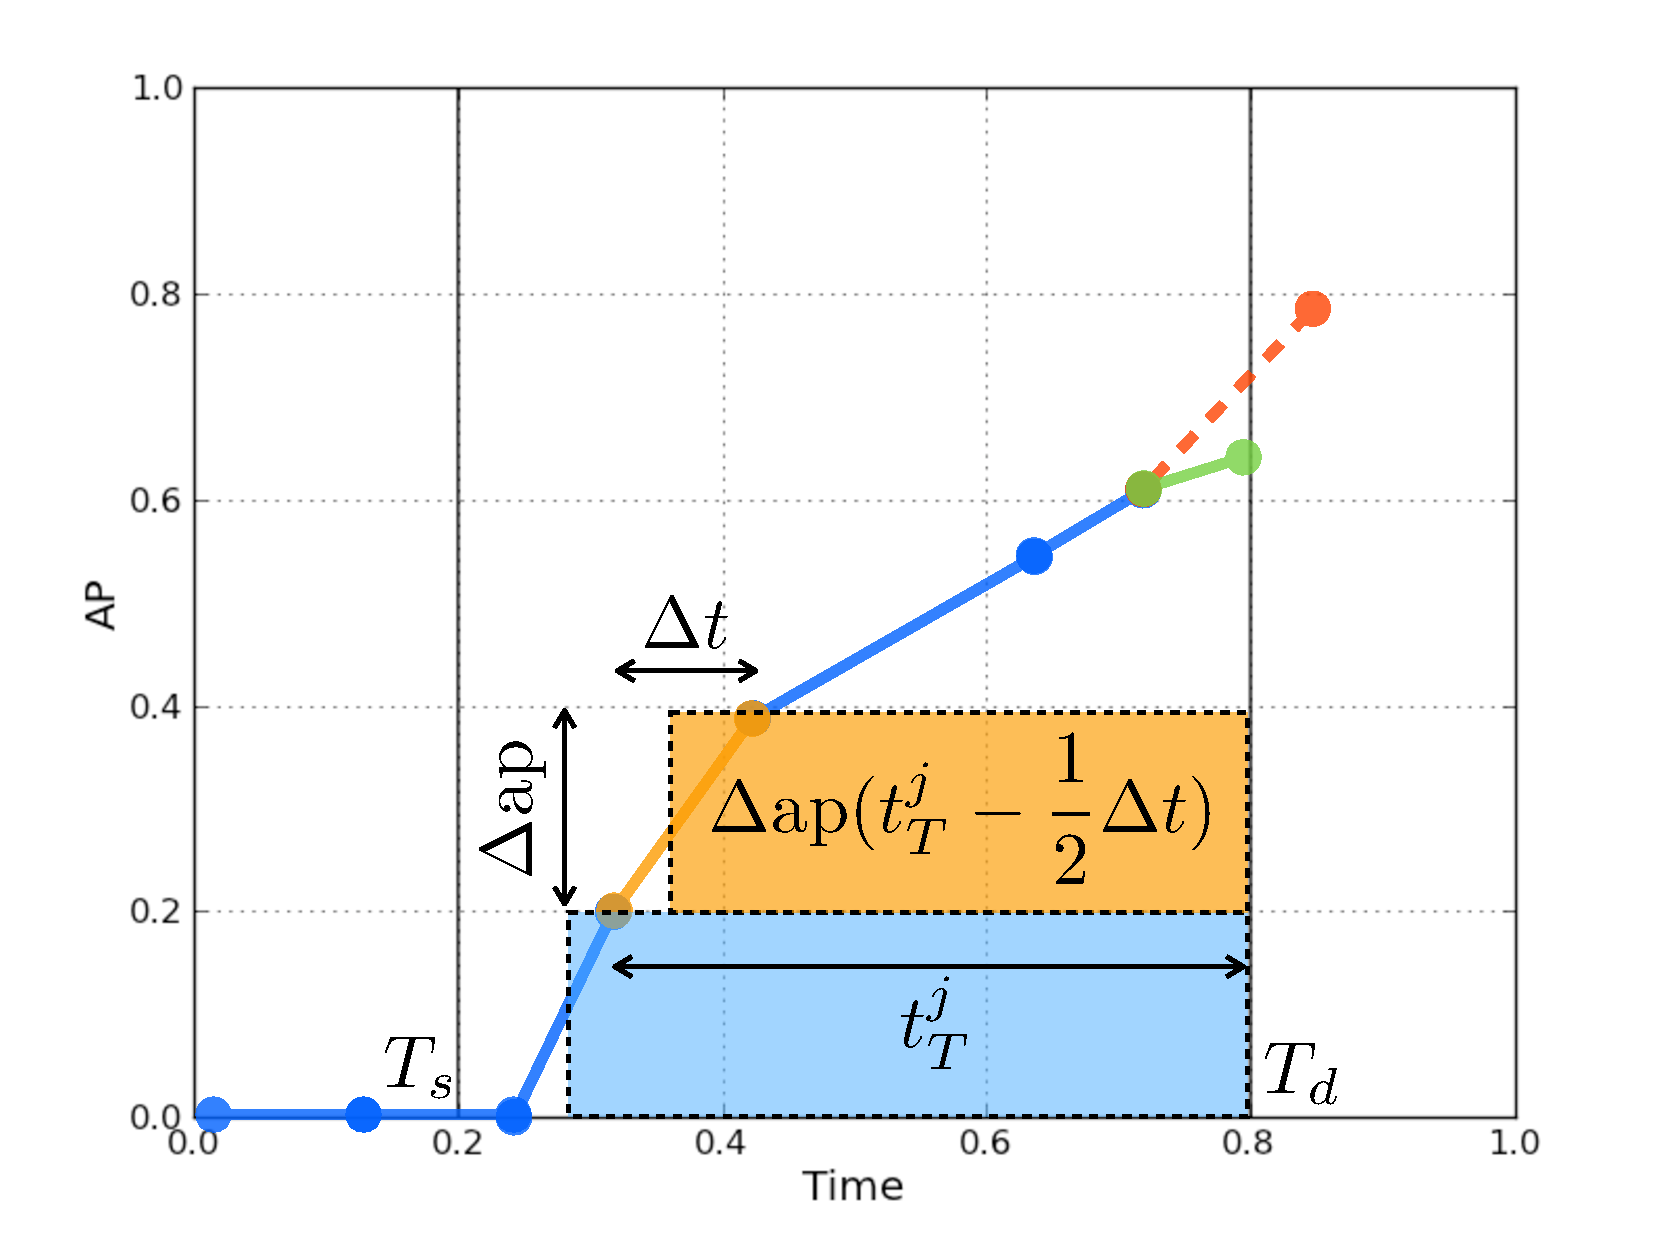
\includegraphics[width=\linewidth]{../../../2011-2012/figures/apvst_expl.pdf}
\caption{
    Graphical representation of the reward function.
}\label{fig:det_rewards}
\end{subfigure}
%
\begin{subfigure}[b]{.48\linewidth}
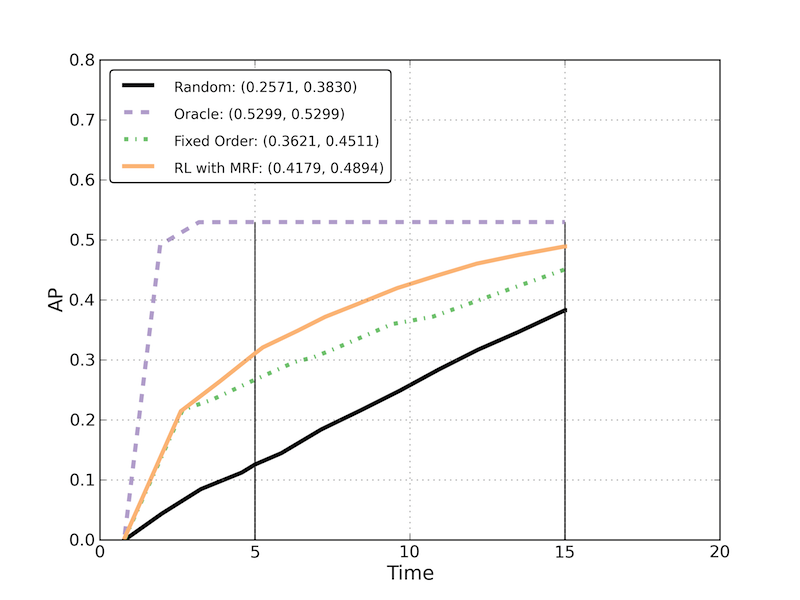
\includegraphics[width=\linewidth]{../../../2011-2012/figures/final1_515.png}
\caption{
    AP vs. Time curves for Random, Oracle, the Fixed Order baseline, and our best-performing policy.
}\label{fig:det_results1}
\end{subfigure}
\end{figure}


\PM{Baselines}
We establish the first baseline for our system by selecting actions randomly at each step.
As shown in \autoref{fig:det_results1}, the \textbf{Random} policy results in a roughly linear gain of AP vs. time.
This is expected: the detectors are capable of obtaining a certain level of performance; if half the detectors are run, the expected performance level is half of the maximum level.
To establish an upper bound on performance, we plot the \textbf{Oracle} policy, obtained by re-ordering the actions at the end of each detection episode in the order of AP gains they produced.
We consider another baseline: selecting actions in a fixed order based on the value they bring to the AP vs. Time evaluation, which is roughly proportional to their occurrence probability.
We refer to this as \textbf{Fixed Order}.

\PM{Ours}
Then there are instantiations of our method, as described in the previous section : \textbf{RL w/ Direct} inference and \textbf{RL w/ MRF} inference.
As the \textbf{MRF} model consistently outperformed \textbf{Direct} by a small margin, we report results for that model only.
In additional to the detector actions, we include a scene-level GIST feature that updates the posterior probabilities of all classes.
This is considered one action, takes about $0.3$ seconds, and brings another boost in performance.
The results are shown in \autoref{tab:det_results}.

\begin{figure}[h!]
\centering
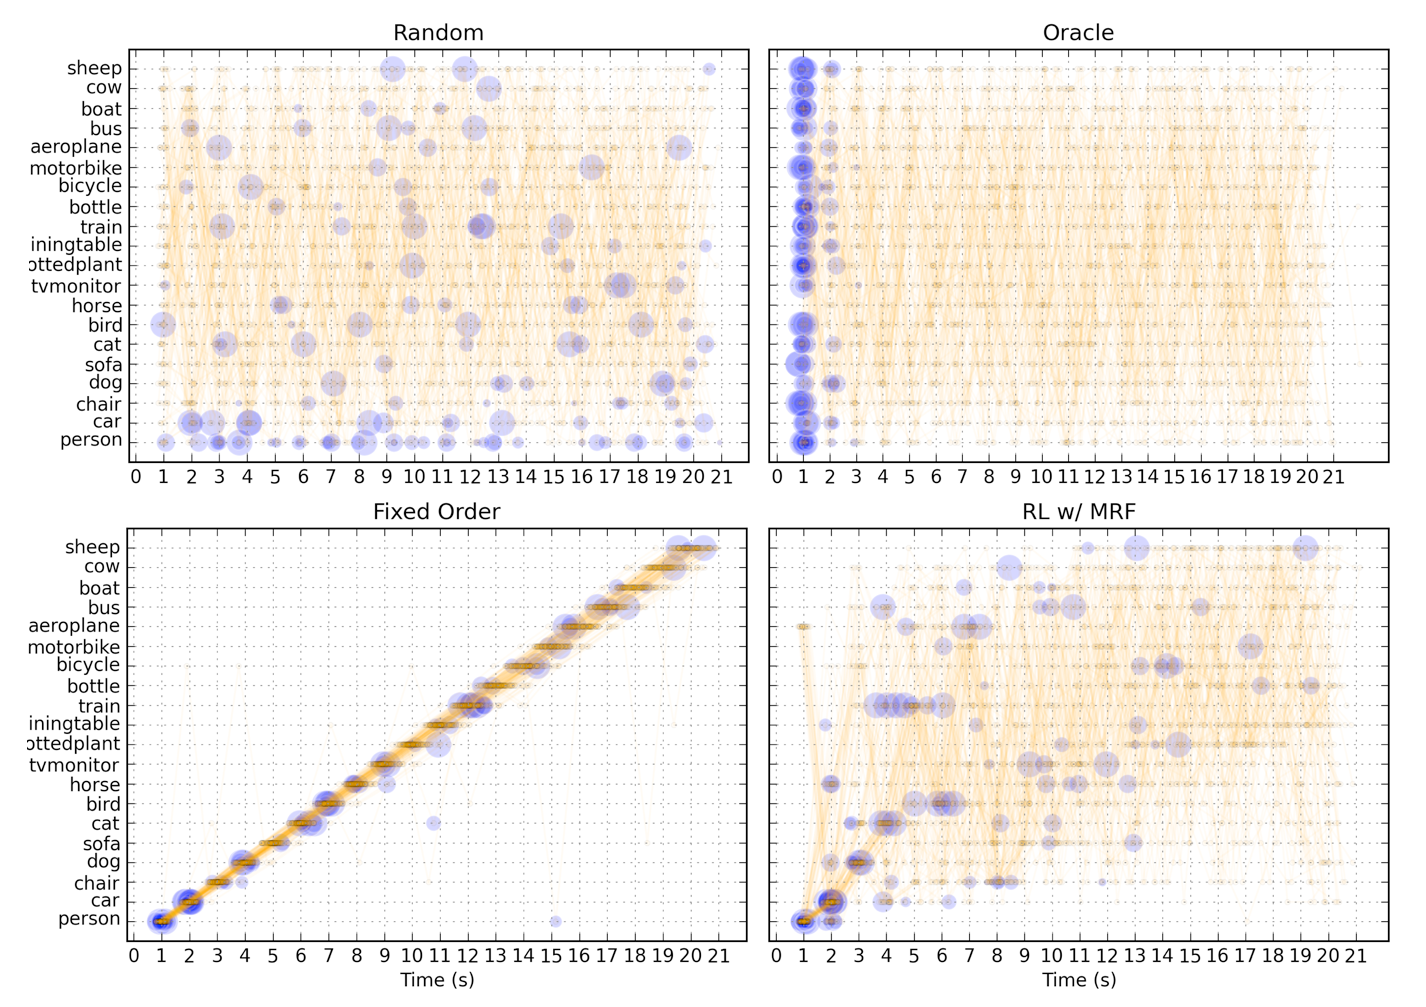
\includegraphics[width=\linewidth]{../../../2011-2012/figures/trajectories.pdf}
\caption[
Visualizing action trajectories of different object detection policies.]{
Visualizing the action trajectories of different policies.
Action selection traces are plotted in orange over many episodes; the size of the blue circles correspond to the increase in AP obtained by the action.
We see that the \textbf{Random} policy selects actions and obtains rewards randomly, while the \textbf{Oracle} policy obtains all rewards in the first few actions.
The \textbf{Fixed Order} policy selects actions in a static optimal order.
Our \textbf{RL w/ MRF} policy does not stick a static order but selects actions dynamically to maximize the rewards obtained early on.
}
\label{fig:trajectories}
\end{figure}


\PM{Trajectories}
In \autoref{fig:det_results1}, we can see that due to the dataset bias, the fixed-order policy performs well at first, as the person class is disproportionately likely to be in the image, but is significantly overtaken by our model as execution goes on and more rare classes have to be detected.
It is additionally informative to consider the action trajectories of different policies in \autoref{fig:trajectories}.
In contrast to the fixed order policy, our method is clearly dynamic, jumping from action to action based on the observations obtained from previous actions.

\begin{figure}[h!]
\centering
\begin{subfigure}[t]{.8\linewidth}
    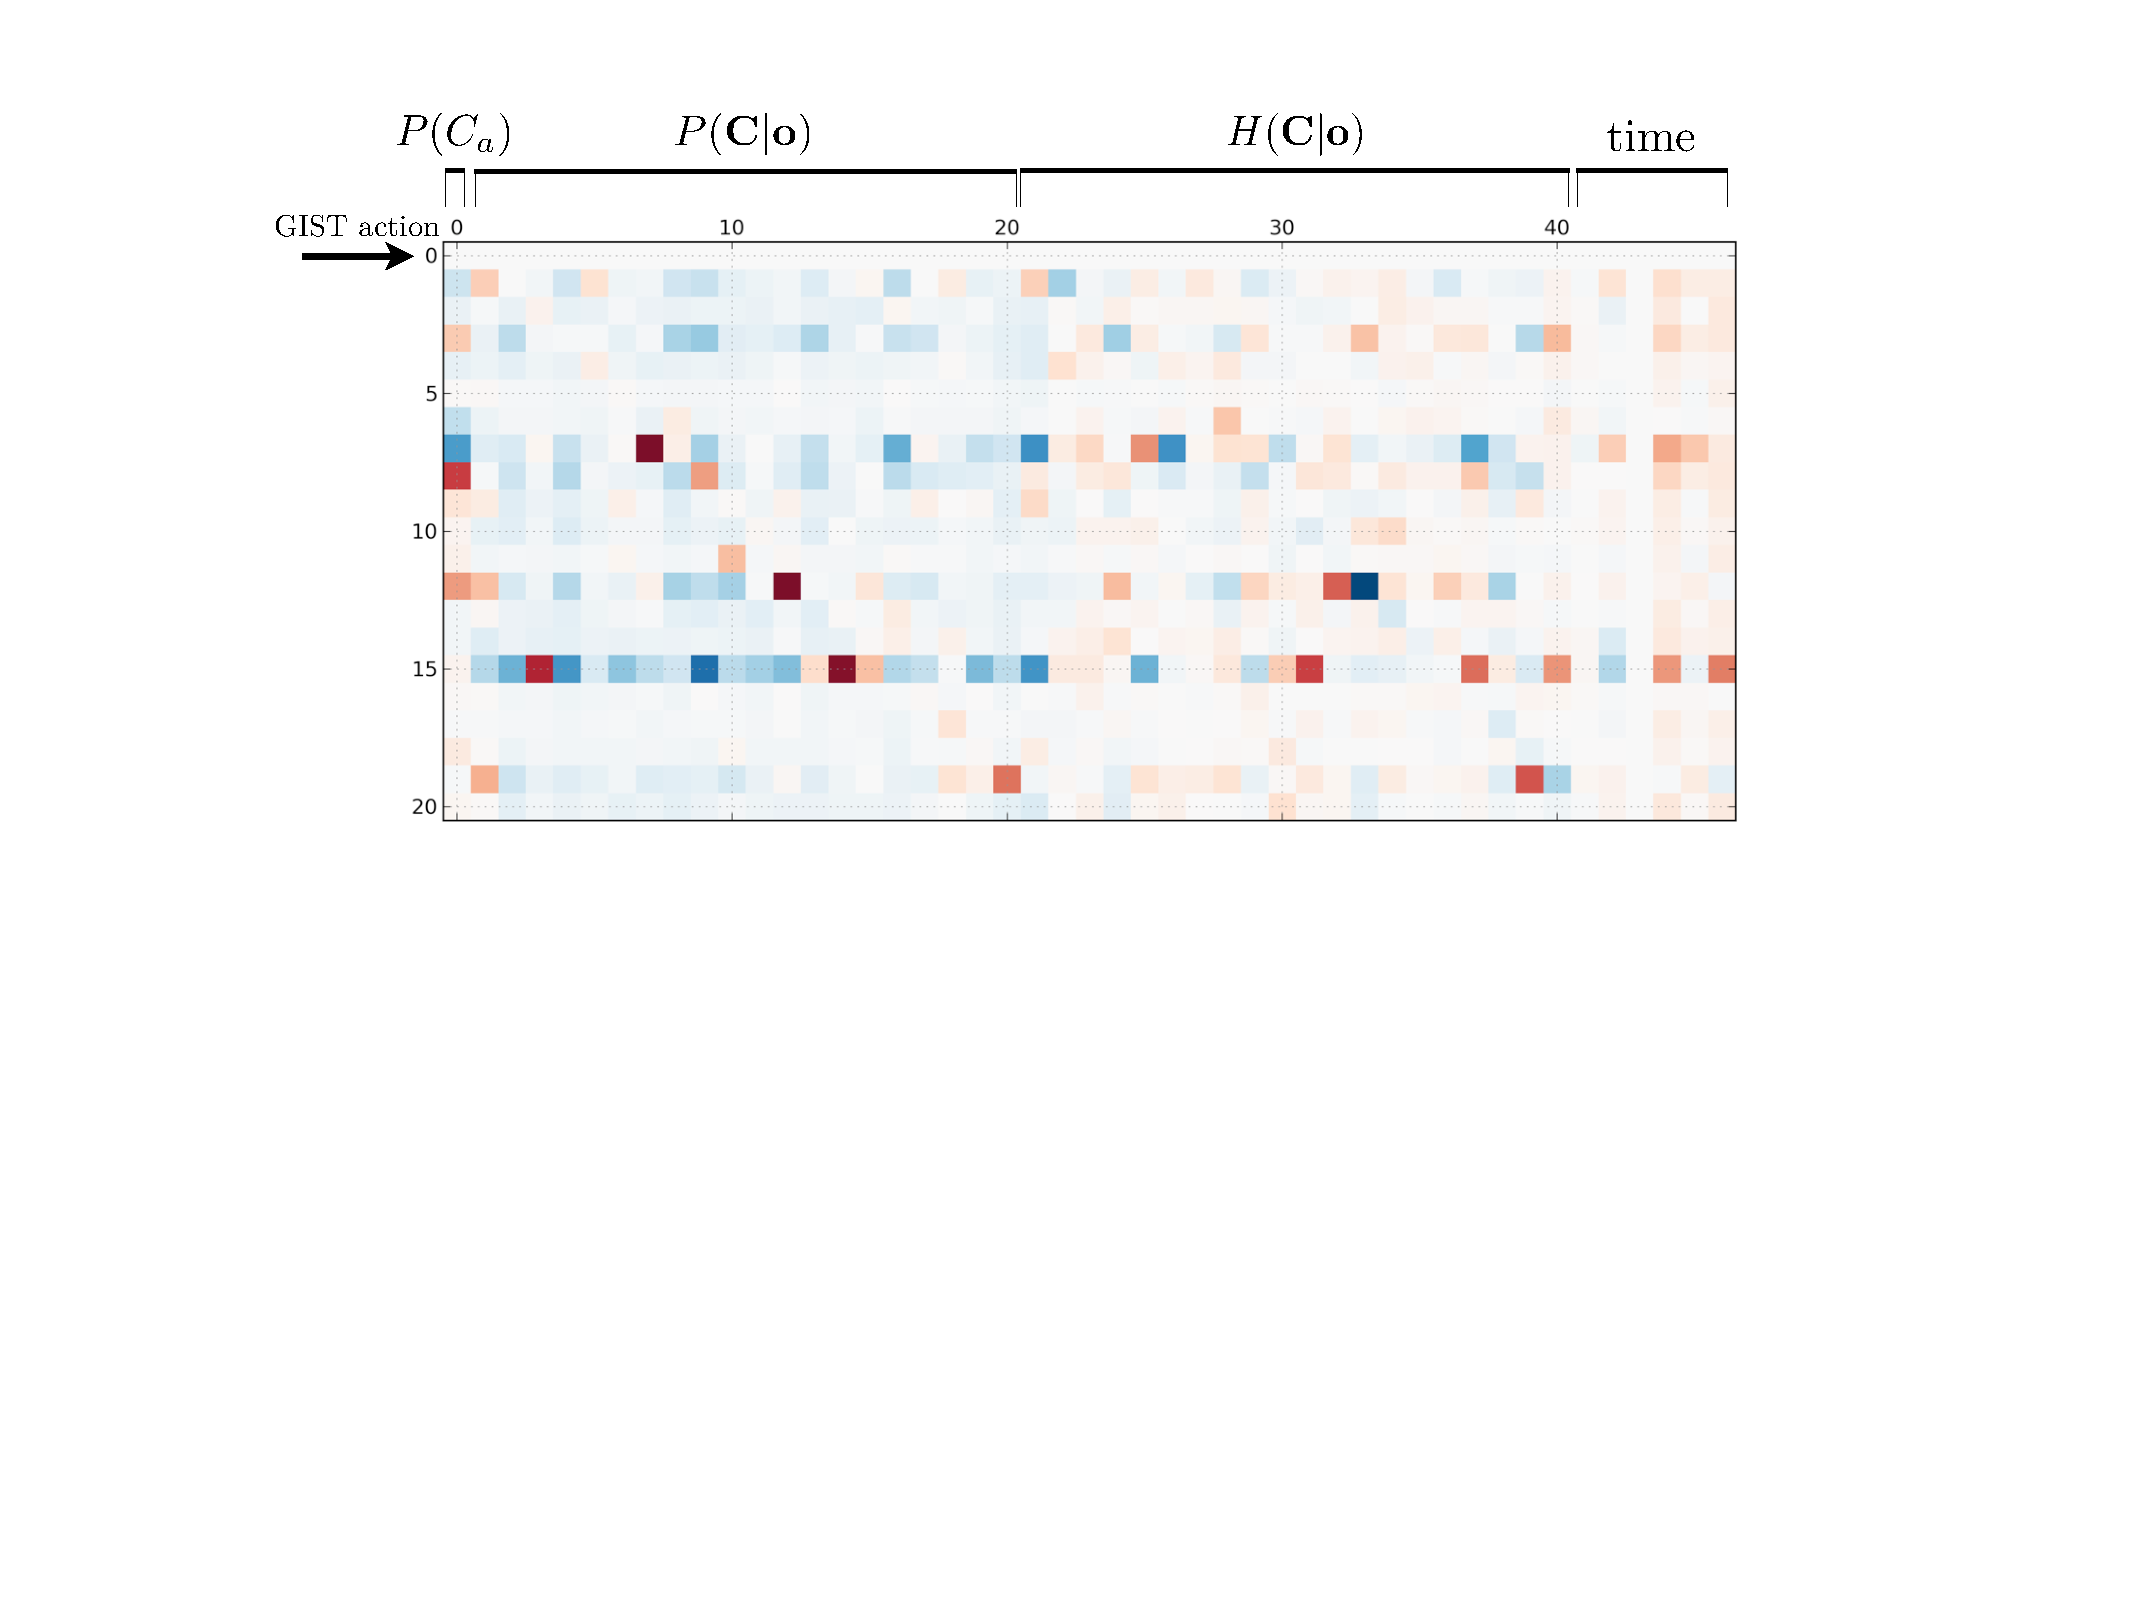
\includegraphics[width=\linewidth]{../../../2011-2012/figures/weights_greedy}
    \caption{Greedy}
\end{subfigure}\\
\begin{subfigure}[t]{.8\linewidth}
    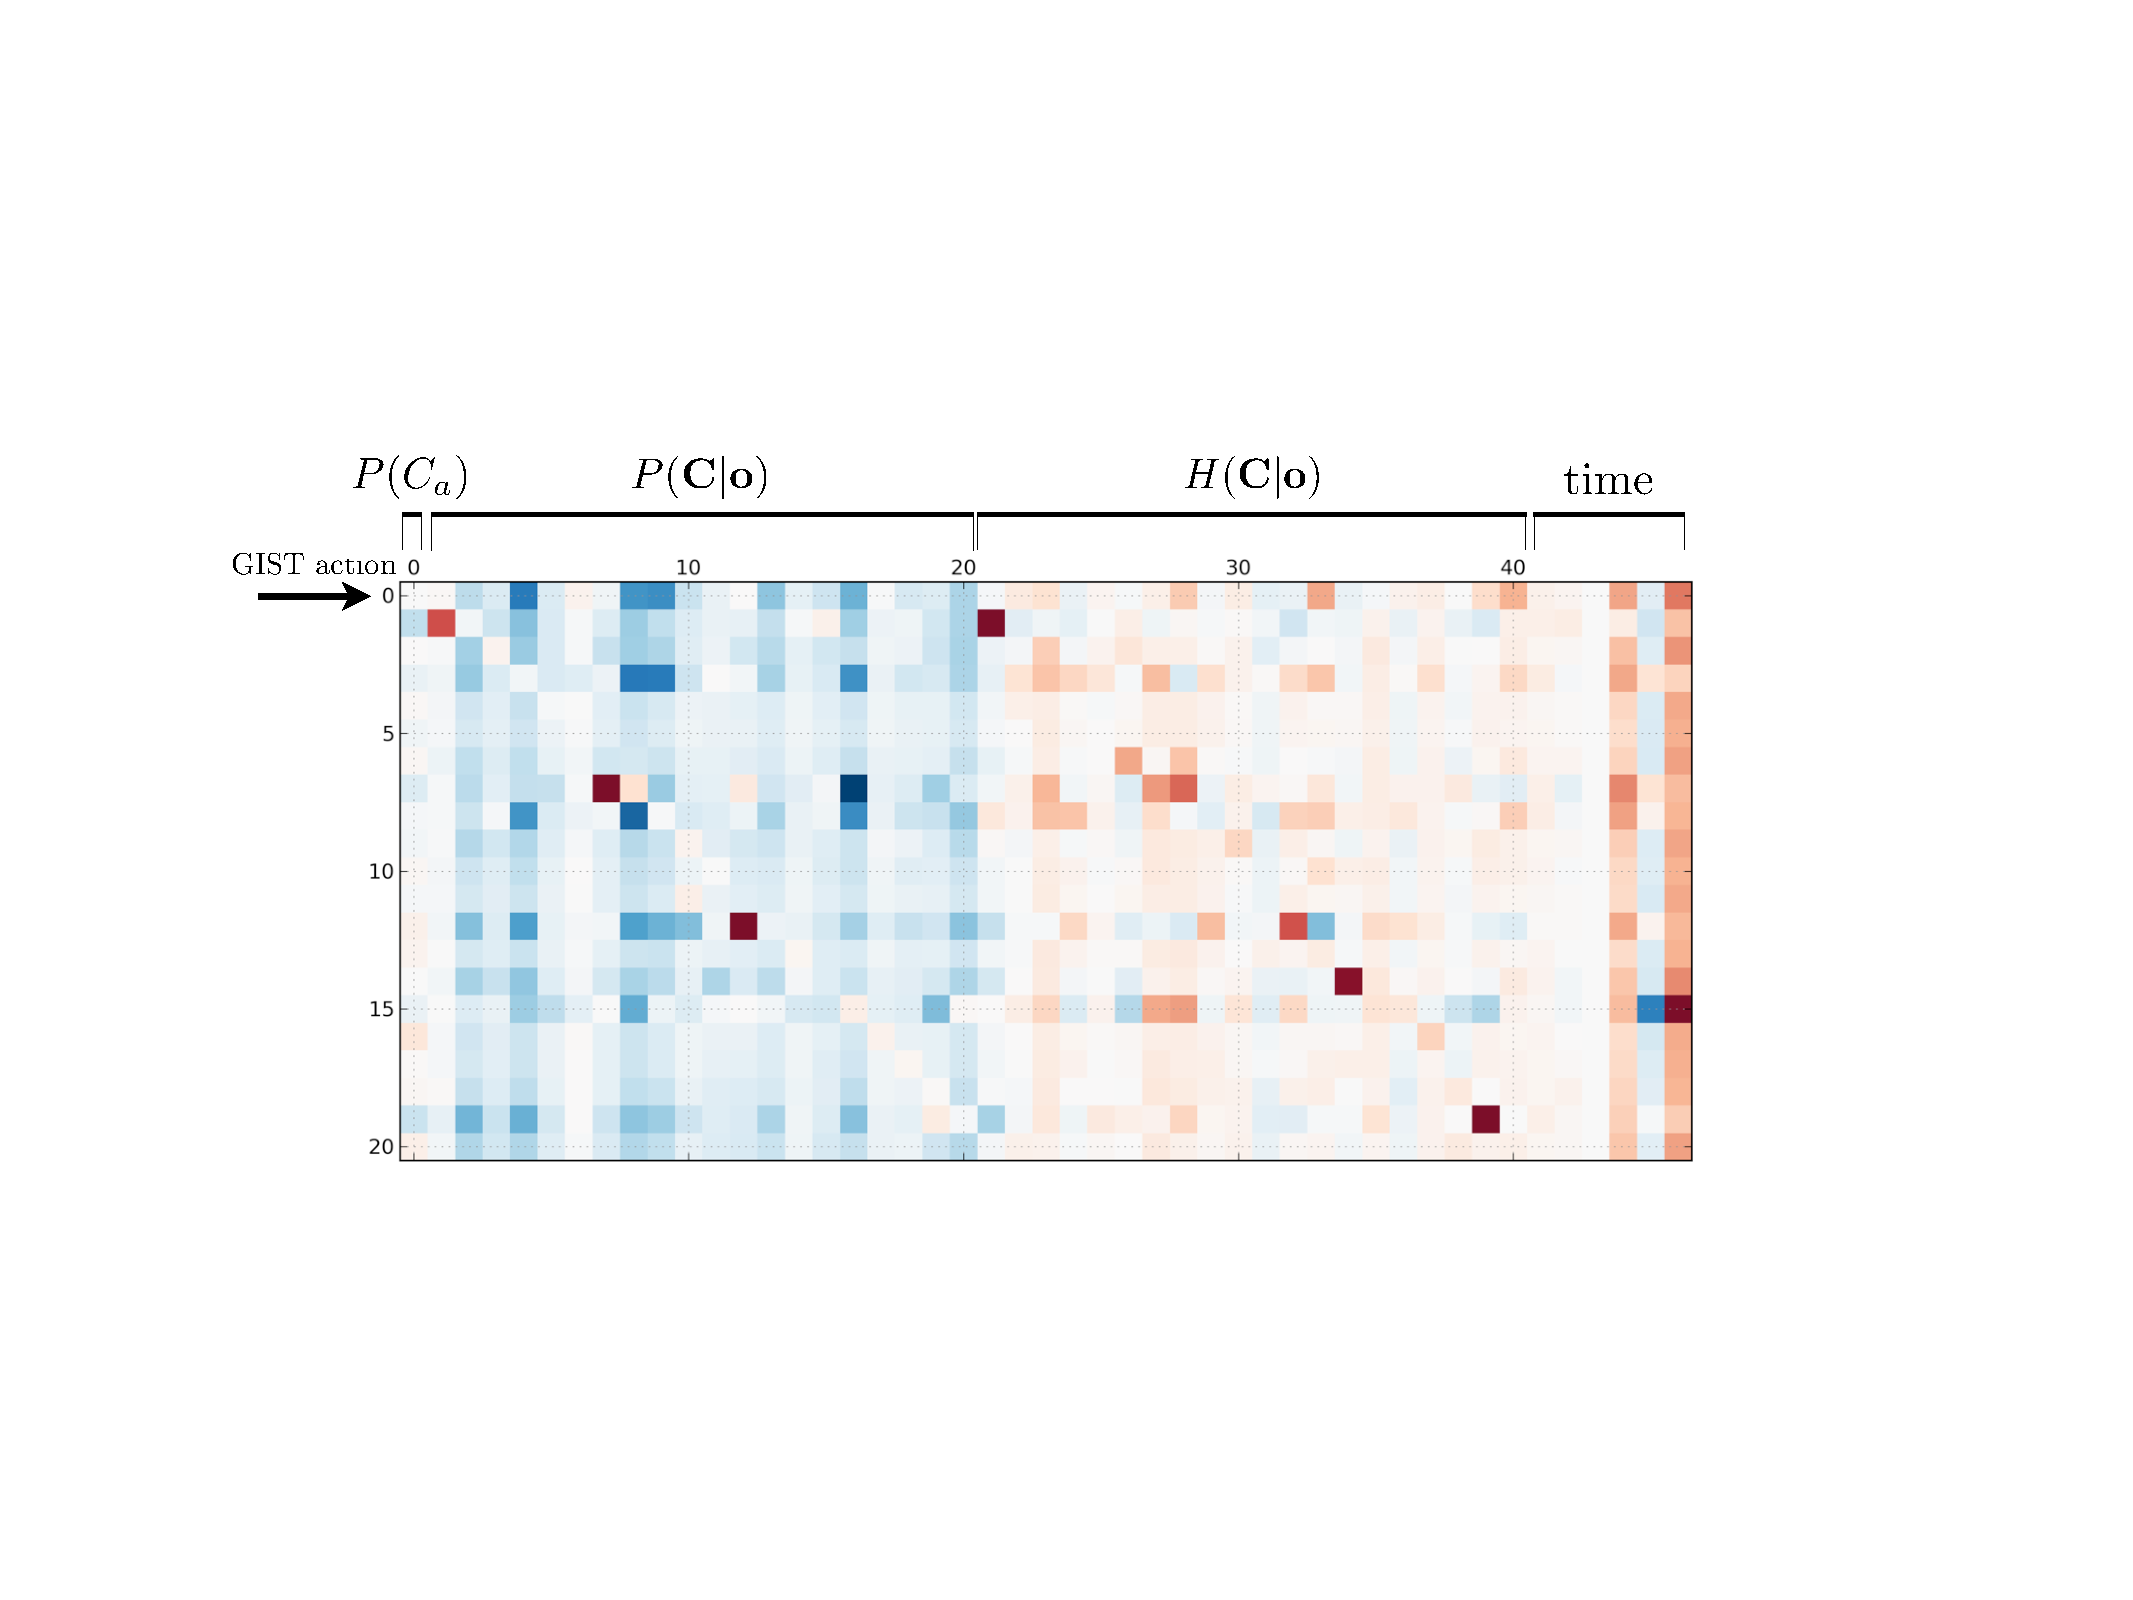
\includegraphics[width=\linewidth]{../../../2011-2012/figures/weights_rl}
    \caption{Reinforcement Learning}
\end{subfigure}
\caption[Learned policy weights for the detection approach.]{
Learned policy weights $\theta_\pi$ (best viewed in color: red corresponds to positive, blue to negative values).
The first row corresponds to the scene-level action, which does not generate detections itself but only helps reduce uncertainty about the contents of the image.
Note that in the greedy learning case, this action is learned to never be taken, but it is shown to be useful in the reinforcement learning case.
}
\label{fig:det_weights}
\end{figure}


\PM{Learned weights}
As an illustration, we visualize the learned weights on features as described in \autoref{sec:det_features} in \autoref{fig:det_weights}.
The weights are reshaped such that each row shows the weights learned for an action, with the top row representing the scene context action and then next $20$ rows corresponding to the PASCAL VOC class detector actions.
We note that the GIST action is learned to never be taken in the greedy ($\gamma=0$) setting, but is learned to be taken with a higher value of $\gamma$.

\begin{table}[t]
\caption{The areas under the AP vs. Time curve for different experimental conditions.}
\label{tab:det_results}
\centering
\begin{tabular}{|c|c|c|c|c|c|}
\hline
Bounds & Random & Fixed Order & RL        & RL w/ GIST         & Oracle \\ \hline
(0,20) & 0.250  & 0.342       & 0.378     & \textbf{0.382}  & 0.488 \\
(0,10) & 0.119  & 0.240       & 0.266     & \textbf{0.267}  & 0.464 \\
(5,15) & 0.257  & 0.362       & 0.418     & \textbf{0.420}  & 0.530 \\ \hline
\end{tabular}
\end{table}
